\documentclass[tikz,border=10pt]{standalone}

\begin{document}
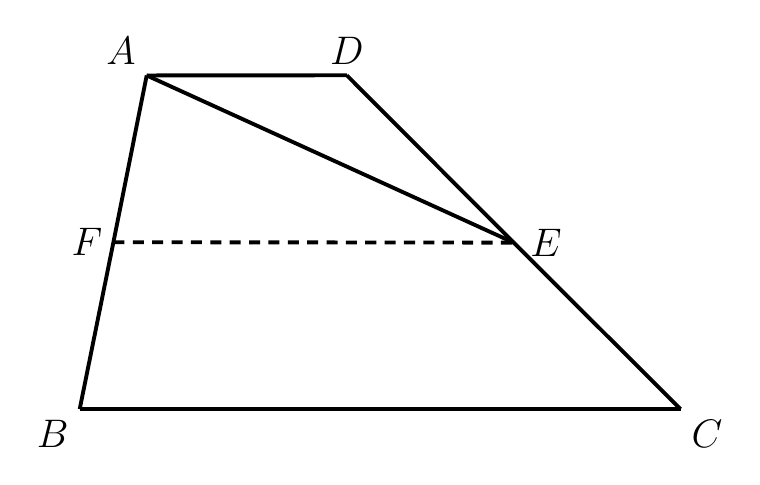
\begin{tikzpicture}[line width=1.4pt, line join=round,
  every node/.style={font=\fontsize{14}{16.8}\selectfont}]
\coordinate (A) at (-2.978,2.130);
\coordinate (B) at (-3.829,-2.108);
\coordinate (C) at (3.802,-2.108);
\coordinate (D) at (-0.437,2.132);
\coordinate (E) at (1.682,0.007);
\coordinate (F) at (-3.401,0.012);



\draw (A) -- (D);      
\draw (D) -- (E);      
\draw (E) -- (C);      
\draw (C) -- (B);      
\draw (B) -- (F);      
\draw (F) -- (A);      
\draw (A) -- (E);      


\draw[dash pattern=on 4pt off 3pt] (F) -- (E);

\node[above left] at (A) {$A$};
\node[above] at (D) {$D$};
\node[below left] at (B) {$B$};
\node[below right] at (C) {$C$};
\node[left] at (F) {$F$};

\node[right, xshift=2pt] at (E) {$E$};
\end{tikzpicture}
\end{document}
